%=======================================================================
% P-LENS — Plasticity-pressure-driven Law Enforcement of Network Structure
% Springer LNCS template (llncs.cls). Class project paper.
%
% Build:  pdflatex main ; bibtex main ; pdflatex main ; pdflatex main
% The class file llncs.cls and bibliography style splncs04.bst are included
% in this folder (official Springer LNCS package).
%=======================================================================
\documentclass[runningheads]{llncs}

\usepackage[T1]{fontenc}
\usepackage[utf8]{inputenc}
\usepackage{graphicx}
\usepackage{amsmath}
\usepackage{amssymb}
\usepackage{booktabs}
\usepackage{array}
\usepackage{url}
\usepackage[dvipsnames]{xcolor}
\usepackage{tikz}
\usetikzlibrary{arrows.meta,positioning}
\usepackage{tcolorbox}
\tcbuselibrary{skins,breakable}
\usepackage{enumitem}
\usepackage{fancyhdr}

\graphicspath{{figures/}}

%--- Soft VIT-AP themed palette ---------------------------------------
\definecolor{vitblue}{RGB}{0,61,120}
\definecolor{vitaccent}{RGB}{212,175,55}
\definecolor{vitlight}{RGB}{236,241,248}

%--- Colored section headings (native llncs layout, recolored) --------
\makeatletter
\renewcommand\section{\@startsection{section}{1}{\z@}%
  {-16\p@ \@plus -4\p@ \@minus -4\p@}%
  {8\p@ \@plus 4\p@ \@minus 4\p@}%
  {\normalfont\large\bfseries\boldmath\color{vitblue}%
   \rightskip=\z@ \@plus 8em\pretolerance=10000}}
\renewcommand\subsection{\@startsection{subsection}{2}{\z@}%
  {-15\p@ \@plus -4\p@ \@minus -4\p@}%
  {7\p@ \@plus 4\p@ \@minus 4\p@}%
  {\normalfont\normalsize\bfseries\boldmath\color{vitblue}%
   \rightskip=\z@ \@plus 8em\pretolerance=10000}}
%--- Each section starts on a fresh page -----------------------------
\let\plens@section\section
\renewcommand\section{\clearpage\plens@section}
\makeatother

%--- Roomier display math (formulas were too cramped) -----------------
\setlength{\abovedisplayskip}{10pt plus 3pt minus 3pt}
\setlength{\belowdisplayskip}{10pt plus 3pt minus 3pt}
\setlength{\abovedisplayshortskip}{6pt plus 2pt}
\setlength{\belowdisplayshortskip}{6pt plus 2pt}

%--- Soft running header / footer -------------------------------------
\pagestyle{fancy}
\fancyhf{}
\renewcommand{\headrulewidth}{0.4pt}
\renewcommand{\footrulewidth}{0pt}
\fancyhead[L]{\footnotesize\color{vitblue}\itshape P-LENS}
\fancyhead[R]{\footnotesize\color{vitblue}\thepage}

%--- Slightly tighter, tasteful lists ---------------------------------
\setlist[itemize]{topsep=3pt,itemsep=2pt,parsep=0pt,leftmargin=1.4em}

%--- Fewer overfull boxes without visibly loosening text --------------
\setlength{\emergencystretch}{2em}

%--- Ragged, wrap-friendly table columns ------------------------------
\newcolumntype{L}[1]{>{\raggedright\arraybackslash}p{#1}}

\begin{document}

\title{P-LENS: Plasticity-Pressure-Driven Law Enforcement of\\
Evolving Network Structure with Machine-Learning-Guided\\
Budgeted Topology Mutations}

\titlerunning{P-LENS: Plasticity-Pressure-Driven Topology Adaptation}

\author{Team~5\inst{1}}

\authorrunning{Team~5}

\institute{VIT-AP University, Amaravati, Andhra Pradesh, India\\
\email{team5@vitapstudent.ac.in} % replace with your own address
}

\maketitle

\begin{abstract}
We present \emph{P-LENS} (Plasticity-pressure-driven Law Enforcement of Network
Structure), a simulation framework for an evolving communication network whose
topology is continuously adapted while it is under load, failures and recovery.
P-LENS couples four ideas: (i) a per-node \emph{state and structural drift
monitor} that observes topology drift, traffic mismatch, congestion and
resilience deficiency; (ii) a scalar \emph{plasticity pressure} that fuses these
indicators and accumulates unresolved pressure as \emph{plasticity debt}; (iii) a
global \emph{mutation budget} that throttles how much structural change the
network is allowed to perform; and (iv) a \emph{mutation field} that scores
candidate ADD/PRUNE/REWIRE actions and feeds a constraint-aware selector. Each
accepted mutation is evaluated after a delay $k$ with a counterfactual shadow
re-run, and the resulting gain updates a per-edge \emph{mutation credit} that
strengthens or suppresses similar future actions. A GRU sequence model forecasts
the next window's attack/normal stress from sliding windows of aggregate flow
features and modulates the offered-load intensity target. We evaluate P-LENS
against static, random-adaptive and greedy baselines under common random
numbers, and ablate each mechanism. On a 24-node small-world topology driven by
synthetic and CIC-IDS2017-derived demand, P-LENS yields lower mean latency than
the static and greedy baselines while performing far fewer mutations than the
random-adaptive baseline; ablating the debt mechanism collapses adaptation,
and ablating the budget drives mutation to its per-step ceiling. We discuss the
framework, its equations, the experimental protocol, and a candid list of
threats to validity, including several integration caveats in the current
implementation.

\keywords{Evolving networks \and Self-healing networks \and Adaptive topology
\and Network resilience \and Recurrent neural networks \and Network simulation.}
\end{abstract}

\begin{center}
\IfFileExists{figures/vitap-logo.png}{%
  
\includegraphics[width=0.36\textwidth]{figures/vitap-logo.png}%
}{%
  {\Large\bfseries\color{vitblue}VIT-AP University}%
}
\end{center}

\vspace{-0.3em}
\begin{tcolorbox}[enhanced,colback=vitlight,colframe=vitblue,
  boxrule=0.6pt,arc=2.5pt,left=6pt,right=6pt,top=4pt,bottom=5pt]
\centering\small
{\color{vitblue}\textbf{Team~5 --- Project Members}}\\[5pt]
\begin{tabular}{ll}
\toprule
\textbf{Name} & \textbf{Roll number}\\
\midrule
Bellana Sai           & 24bca7931\\
V.~Sai Prakash Yadav  & 24bce8525\\
K.~Niharika           & 24BCE8516\\
Sarvesh               & 24bcw7042\\
K.~Sri Lakshmi        & 24BCS7106\\
\bottomrule
\end{tabular}
\end{tcolorbox}

%-=-=-=-=-=-=-=-=-=-=-=-=-=-=-=-=-=-=-=-=-=-=-=-=-=-=-=-=-=-=-=-=-=-=-=-
\section{Introduction}
\label{sec:intro}

Communication networks increasingly have to operate in non-stationary
conditions: traffic demand shifts, links and nodes fail, and the ``best''
topology is not a fixed design point but a moving target. Fixed topologies that
are optimal for one traffic profile are brittle when demand moves or when parts
of the network fail, while fully reactive schemes that rewire at every
opportunity pay a stability price in the form of churn and transient
disruption.

This paper studies a middle ground: an \emph{evolving-topology} network that is
allowed to change its structure, but only when there is a measurable, unresolved
reason to do so, and only within a budget. We propose \emph{P-LENS}
(Plasticity-pressure-driven Law Enforcement of Network Structure). The name
reflects the central metaphor: the network has \emph{plasticity} (the freedom to
change shape), it is driven by \emph{pressure} (accumulated stress), and the
amount of change is \emph{enforced} by a global budget.

P-LENS is organised as a closed loop around four graph-level state variables:
topology drift $D$, traffic mismatch $F$, congestion $C$ and resilience
deficiency $R$. These are fused per node into a plasticity pressure $PP$, whose
unresolved part accumulates as plasticity debt $PD$. A mutation budget $B$
gates a mutation field $MF$ that scores candidate structural operations
(ADD/PRUNE/REWIRE of an edge). A constraint-aware selector applies the highest
scoring, feasible operations, and a delayed counterfactual evaluation assigns
each accepted operation a gain $G$ that feeds back as mutation credit $MC$ and,
together with the debt, into the next step's budget. A lightweight recurrent
model forecasts the next traffic window's stress class and modulates the offered
load.

\paragraph{Contributions.}
\begin{itemize}
\item We define an evolving-network simulation loop with explicit, documented
formulas for indicators, pressure, debt, budget, mutation field, selection,
delayed evaluation and credit (\S\ref{sec:framework}).
\item We show how to keep the adaptation \emph{auditable}: every rejected
candidate is logged with a machine-readable reason, and every accepted mutation
carries its counterfactual gain.
\item We provide a reproducible experimental protocol with common random numbers,
confidence intervals and paired non-parametric tests, plus ablations that
isolate each mechanism (\S\ref{sec:setup}--\ref{sec:results}).
\item We release the full implementation and report a set of honest limitations,
including integration caveats that affect the machine-learning component
(\S\ref{sec:limitations}).
\end{itemize}

The remainder of the paper is organised as follows.
Section~\ref{sec:related} reviews related work and
Section~\ref{sec:diff} explains how P-LENS differs from it.
Section~\ref{sec:prelim} fixes notation and the network model.
Section~\ref{sec:framework} describes P-LENS.
Section~\ref{sec:setup} presents the experimental setup,
Section~\ref{sec:results} the results, and
Section~\ref{sec:limitations} the threats to validity.
Section~\ref{sec:conclusion} concludes.

%-=-=-=-=-=-=-=-=-=-=-=-=-=-=-=-=-=-=-=-=-=-=-=-=-=-=-=-=-=-=-=-=-=-=-=-
\section{Related Work}
\label{sec:related}

\paragraph{Resilient and self-healing networks.}
The study of networks that degrade gracefully under failure goes back to
distributed-communications work on survivable topologies \cite{baran1964}, and
was later formalised for scale-free and random graphs, where connectivity under
random and targeted failures has explicit thresholds \cite{albert2000,callaway2000}.
Self-healing and autonomic-networking approaches automate fault detection and
reconfiguration \cite{kephart2003,pan2011}. P-LENS shares the goal of resilience
but differs in \emph{what drives change}: rather than reacting to faults alone,
it acts on a composite pressure signal that also includes drift and congestion,
and it explicitly budgets how much structural change is permitted per unit time.

\paragraph{Traffic-aware topology adaptation.}
Software-defined networking makes the control plane programmable and has
enabled traffic-aware routing and topology management \cite{kreutz2015}. Graph
generators such as the Watts--Strogatz small-world and Barab\'asi--Albert
preferential-attachment models \cite{watts1998,barabasi1999} supply the initial
topologies used in our study. Our mutation vocabulary (edge add/prune/rewire)
and the constraint set (degree bounds, connectivity, a local-connectivity
target) are standard in this literature; our focus is the \emph{control law}
that decides when a change is worth making.

\paragraph{Learning traffic and attack signals.}
Intrusion-detection datasets such as CIC-IDS2017 \cite{sharafaldin2018} and
UNSW-NB15 \cite{moustafa2015} provide labelled flow records. Recurrent sequence
models, in particular gated recurrent units (GRUs) \cite{cho2014} and LSTMs
\cite{hochreiter1997}, are widely used for temporal traffic and intrusion
classification. P-LENS uses a small GRU \cite{paszke2019} strictly as a
\emph{forecaster whose output modulates the offered-load intensity target}; it
never chooses topology operations directly.

%-=-=-=-=-=-=-=-=-=-=-=-=-=-=-=-=-=-=-=-=-=-=-=-=-=-=-=-=-=-=-=-=-=-=-=-
\section{How P-LENS Differs from Existing Work}
\label{sec:diff}

We are explicit about novelty: every individual \emph{ingredient} of P-LENS is
known. Adaptive and self-healing reconfiguration, traffic-aware topology
control, edge add/prune/rewire operations, degree and connectivity constraints,
and recurrent traffic forecasting all appear in prior work. What is distinctive
is how these are \emph{combined into one control loop with explicit accounting}
of why, whether, and how much the topology should change. We contrast the design
axes below; Table~\ref{tab:diff} summarises them.

\paragraph{Composite, accumulated trigger.}
Most self-healing schemes fire on a single signal---a fault, an SLA violation or
a congestion threshold. P-LENS fuses four indicators, drift $D$, traffic
mismatch $F$, congestion $C$ and resilience deficiency $R$, into a per-node
pressure, and then integrates the \emph{unresolved} part over time as debt. A
node that has been marginal for a long time is therefore treated differently
from one that spiked briefly, which single-signal triggers cannot express.

\paragraph{Budgeted change.}
Reconfiguration is usually either unpriced (act whenever a rule fires) or
bounded only by a hard per-step cap. P-LENS makes global change a first-class,
refillable \emph{resource} that is spent by operations, earned back from debt
and demonstrated benefit, and penalised by stability cost. The budget thus
trades adaptation against churn explicitly, and the \texttt{no\_budget}
ablation (\S\ref{sec:res-ablations}) shows this mechanism is load-bearing.

\paragraph{Delayed, counterfactual credit assignment.}
Many adaptive schemes are open-loop: they act but never measure whether the
action helped. P-LENS evaluates each accepted mutation $k$ steps later by
re-routing the same demand on a shadow topology with the mutation reversed, and
folds the resulting gain into a per-edge credit that biases future scores
(Eq.~\ref{eq:credit}). This is a cheap, simulation-only form of credit
assignment for topology actions, absent from rule-based reconfiguration.

\paragraph{Auditable, constraint-aware selection.}
Instead of a monolithic policy, selection is a ranked, constraint-filtered
process in which every rejected candidate is recorded with a machine-readable
reason (\texttt{degree\_cap}, \texttt{would\_disconnect}, \texttt{cooldown},
\dots). This makes the controller's decisions inspectable---unusual for learned
or heuristic controllers, which tend to be opaque.

\paragraph{Narrow, non-authoritative machine learning.}
In reinforcement-learning approaches the learned model \emph{is} the policy. In
P-LENS the GRU is deliberately quarantined: it forecasts traffic stress and only
modulates the offered-load intensity target; it never selects operations. This
keeps the structural control law interpretable and lets the learning component
be ablated cleanly, at the current cost of a weak coupling
(\S\ref{sec:limitations}).

\paragraph{What is new versus assembled (honest summary).}
The mechanisms overlap with prior art and we do not claim an architectural
breakthrough. Our contribution is the specific \emph{composition}: a
pressure/debt/budget loop closed by delayed per-edge credit, mutation volume
treated as a budgeted resource, and an implementation plus evaluation protocol
that makes the composition measurable and its failure modes visible. The
individual pieces are individually replaceable, which is exactly what the
ablation study exploits.

\begin{table}[t]
\caption{Design axes: representative approach classes versus P-LENS.}
\label{tab:diff}
\centering\small
\setlength{\tabcolsep}{4pt}%
\begin{tabular}{L{2.6cm}L{1.7cm}L{2.2cm}L{3.4cm}}
\toprule
Class & Trigger & Change control & Main gap P-LENS targets\\
\midrule
Static / redundant design & offline, manual & none & cannot react to drift or failures\\
Self-healing autonomic & failures & rule-based, unbounded & single-signal trigger; no mutation budget\\
Traffic engineering (SDN) & congestion / SLA & periodic global optimisation & no accumulated debt; no per-edge credit\\
RL topology control & learned state & policy-imposed & opaque; the ML model is the policy\\
\textbf{P-LENS} & composite $D,F,C,R$ + debt & budgeted, constraint-aware & (this work)\\
\bottomrule
\end{tabular}
\end{table}

%-=-=-=-=-=-=-=-=-=-=-=-=-=-=-=-=-=-=-=-=-=-=-=-=-=-=-=-=-=-=-=-=-=-=-=-
\section{Preliminaries and Network Model}
\label{sec:prelim}

\paragraph{Topology.}
An evolving network is an undirected graph $G_t = (V, E_t)$ with a fixed node
set $V$, $|V| = n$, and a time-varying edge set $E_t$. Edge $e = (u,v)\in E_t$
carries a bandwidth $b_e$, a propagation latency $\ell_e$ and a reliability
$r_e$. Node states track demand, provisioned bandwidth, utilisation, queueing
delay and loss. Failures and recovery are modelled per step: an alive node
fails with probability $p^{\text{node}}_f$, an edge with alive endpoints fails
with probability $p^{\text{edge}}_f$, and a failed element is repaired after a
fixed number of steps. A node failure takes its incident edges down with it;
those edges recover together with the node. Failed elements remain in the
\emph{logical} graph but are invisible to routing and to the monitor, which see
only the \emph{usable} subgraph of alive nodes and non-failed edges.

\paragraph{Demand and routing.}
Each step supplies an $n\times n$ demand matrix $X_t$ (bytes per origin--destination
pair). The matrix is renormalised so that the total demand equals a target
fraction $\iota$ of the \emph{usable} bandwidth:
\begin{equation}
X_t \leftarrow X_t \cdot \frac{\iota \cdot \sum_{e \text{ usable}} b_e}{\sum_{ij} X_t^{ij}} ,
\label{eq:scale}
\end{equation}
which makes $\iota$ (the traffic intensity) a scale-free knob independent of
current failures. Demand is routed along shortest paths under a
congestion-aware weight
\begin{equation}
w_e = \ell_e\,\bigl(1 + \alpha\,\bar{u}_e\bigr) + \epsilon ,
\label{eq:routing}
\end{equation}
where $\bar{u}_e$ is the previous pass's utilisation, $\alpha$ is the
congestion sensitivity and $\epsilon$ breaks ties. Routing runs in two passes:
a first pass estimates $\bar{u}_e$, the second places the final load.

\paragraph{Bottleneck delivery and delay.}
For a flow traversing a path $P$, the delivered share is its bottleneck share
times the path reliability,
\begin{equation}
\text{share}(P) = \min\!\Bigl(1,\ \min_{e\in P} \tfrac{\mu}{\lambda_e}\Bigr)\prod_{e\in P} r_e ,
\label{eq:share}
\end{equation}
with $\mu$ a service-rate proxy and $\lambda_e$ the placed load. The normalised
M/M/1 queue term on an edge is
\begin{equation}
q_e =
\begin{cases}
\min\!\bigl(1,\ \tfrac{1}{20}(\tfrac{\mu}{\mu-\lambda_e}-1)\bigr), & \lambda_e < \mu,\\[2pt]
1, & \lambda_e \ge \mu \ \text{(saturated)},
\end{cases}
\label{eq:queue}
\end{equation}
and the latency of a delivered flow is the sum of $\ell_e + q_e$ over its path,
averaged over delivered bytes. Network throughput is the delivered share of
demand and loss is its complement.

%-=-=-=-=-=-=-=-=-=-=-=-=-=-=-=-=-=-=-=-=-=-=-=-=-=-=-=-=-=-=-=-=-=-=-=-
\section{The P-LENS Framework}
\label{sec:framework}

Figure~\ref{fig:loop} summarises one simulation step. We now describe each block
and give its formula. All thresholds and weights are configuration parameters
(Table~\ref{tab:config}); every equation below is a design choice rather than a
claim imported from prior work.

\begin{figure}[t]
\centering
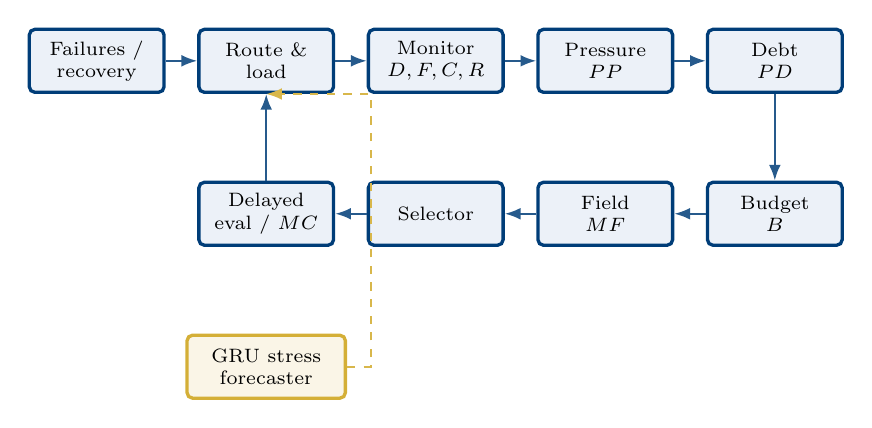
\begin{tikzpicture}[
  font=\scriptsize,
  box/.style={draw=vitblue,very thick,rounded corners=2pt,fill=vitlight,
              align=center,inner sep=3pt,minimum height=8mm,text width=15mm},
  mlbox/.style={draw=vitaccent,very thick,rounded corners=2pt,
              fill=vitaccent!12,align=center,inner sep=3pt,
              minimum height=8mm,text width=18mm},
  ar/.style={-{Latex[length=2mm]},thick,vitblue!85},
  fb/.style={-{Latex[length=2mm]},thick,dashed,vitaccent!90}
]
%--- top row: physical/structural path (left to right)
\node[box] (fail)  {Failures /\\recovery};
\node[box,right=4mm of fail]  (route) {Route \&\\load};
\node[box,right=4mm of route] (mon)   {Monitor\\$D,F,C,R$};
\node[box,right=4mm of mon]   (pp)    {Pressure\\$PP$};
\node[box,right=4mm of pp]    (pd)    {Debt\\$PD$};
%--- second row: control decisions (right to left)
\node[box,below=11mm of pd]  (bud) {Budget\\$B$};
\node[box,left=4mm of bud]   (mf)  {Field\\$MF$};
\node[box,left=4mm of mf]    (sel) {Selector};
\node[box,left=4mm of sel]   (ev)  {Delayed\\eval / $MC$};
%--- quarantined forecaster
\node[mlbox,below=11mm of ev] (ml) {GRU stress\\forecaster};

\draw[ar] (fail)  -- (route);
\draw[ar] (route) -- (mon);
\draw[ar] (mon)   -- (pp);
\draw[ar] (pp)    -- (pd);
\draw[ar] (pd)    -- (bud);
\draw[ar] (bud)   -- (mf);
\draw[ar] (mf)    -- (sel);
\draw[ar] (sel)   -- (ev);
%--- feedback: delayed credit re-enters the top of the loop
\draw[ar] (ev.north) -- ++(0,4mm) -| (route.south);
%--- quarantined ML path into the offered-load target only
\draw[fb] (ml.east) -- ++(3mm,0) |- (route.south);
\end{tikzpicture}
\caption{The P-LENS control loop (one step). Solid blue arrows are the structural
control path; the dashed gold path is the quarantined machine-learning forecaster,
which modulates only the offered-load intensity $\iota$ of \eqref{eq:scale}.}
\label{fig:loop}
\end{figure}

\subsection{State and structural drift monitor}
\label{sec:monitor}

At each step the monitor computes four per-node indicators, all clipped to
$[0,1]$ on the usable topology.

\paragraph{Topology drift $D_i$.} A blend of neighbourhood change and degree
change against a reference topology (the initial graph):
\begin{equation}
D_i = \tfrac12\bigl(1 - J(\mathcal{N}_i, \mathcal{N}^{\text{ref}}_i)\bigr)
     + \tfrac12\,\frac{|k_i - k^{\text{ref}}_i|}{\max(k_i, k^{\text{ref}}_i, 1)},
\label{eq:drift}
\end{equation}
where $J$ is the Jaccard index and $k_i$ is the usable degree of node $i$.

\paragraph{Traffic mismatch $F_i$.} Imbalance between incident demand $x_i$ and
provisioned bandwidth $b_i$:
\begin{equation}
F_i = \frac{|x_i - b_i|}{\max(x_i, b_i, \varepsilon)} .
\label{eq:mismatch}
\end{equation}

\paragraph{Congestion $C_i$.} A weighted mix of node utilisation $u_i$, the
worst incident link utilisation, the normalised queue term $q_i$ and the node
loss $\rho_i$:
\begin{equation}
C_i = w_u u_i + w_l \max_{e\ni i} u_e + w_q q_i + w_p \rho_i .
\label{eq:cong}
\end{equation}

\paragraph{Resilience deficiency $R_i$.} A blend of local-connectivity
deficiency against a target $\lambda^\star$ (proxied by usable degree) and a
failure-impact term:
\begin{equation}
R_i = a\Bigl(1 - \min\!\bigl(1, \tfrac{\lambda_i}{\lambda^\star}\bigr)\Bigr) + (1-a)\,\psi_i,
\qquad \psi_i = \frac{\sum_j (X^{ij}+X^{ji})}{\sum_{jk} X^{jk}},
\label{eq:resil}
\end{equation}
with $R_i = 1$ if node $i$ is failed.

\subsection{Plasticity pressure}
\label{sec:pressure}

The pressure is the EMA-smoothed, normalised weighted sum of the indicators:
\begin{equation}
\widehat{PP}_i = \frac{\sum_{k\in\{D,F,C,R\}} w_k\,\phi_{k,i}}{\sum_k w_k},
\qquad
PP_i(t) = \rho\,\widehat{PP}_i + (1-\rho)\,PP_i(t{-}1),
\label{eq:pressure}
\end{equation}
where $\phi_k$ are the four indicators and $\rho$ the EMA factor. Pressure
answers ``how stressed is this node right now?''

\subsection{Plasticity debt}
\label{sec:debt}

Debt accumulates pressure that has not yet been relieved by successful
structural change:
\begin{equation}
PD_i(t{+}1) = \mathrm{clip}_{[0,1]}\bigl(\gamma\,PD_i(t) + \alpha\,PP_i(t) - \text{relief}_i\bigr),
\label{eq:debt}
\end{equation}
with decay $\gamma$, accumulation $\alpha$, and $\text{relief}_i$ supplied after
a mutation succeeds. Relief is granted to the mutation's endpoints and their
one-hop neighbours (clipped so no node receives more than one relief unit):
\begin{equation}
\text{relief}_i = \mathrm{clip}\Bigl(\sum_{\text{succ. } m} \mathbb{1}[i \in
\mathcal{T}_m]\cdot \delta_r,\ 0,\ \delta_r\Bigr),
\label{eq:relief}
\end{equation}
where $\mathcal{T}_m$ is the closed one-hop neighbourhood of $m$'s endpoints and
$\delta_r$ the per-mutation relief. Pressure answers ``how stressed is this node
now?''; debt answers ``how long has it been stressed and unresolved?''.

\subsection{Mutation budget}
\label{sec:budget}

A scalar budget $B_t$ limits how much structural change is allowed. It is spent
by operations and refilled from debt and demonstrated benefit, and penalised by
stability cost:
\begin{equation}
B_{t+1} = \mathrm{clip}_{[B_{\min}, B_{\max}]}\Bigl(
B_t - \text{spent}_t + \beta\,\overline{PD}_t
+ \eta_g\,\overline{G^+}_t - \eta_s\,\overline{S}_t \Bigr),
\label{eq:budget}
\end{equation}
where $\overline{PD}_t$ is the mean debt, $\overline{G^+}_t$ the mean positive
delayed gain, $\overline{S}_t$ the mean stability cost, $\beta$ the refill rate
and $\eta_g,\eta_s$ the gain/stability weights. A per-operation gate allows an
operation of cost $c$ only if $B_t \ge c$.

\subsection{Mutation field}
\label{sec:field}

The mutation field scores every candidate structural operation $op$ (ADD, PRUNE
or REWIRE) on a candidate edge $(i,j)$:
\begin{equation}
\begin{split}
MF^{op}_{ij} = g(B_t, c_{op})\Bigl(
&w_n\,\text{need}_{ij} + w_d\,\text{debt}_{ij} + w_b\,\text{benefit}^{op}_{ij}\\
&+ w_c\,\text{credit}_{ij} - w_k\,\text{cost}_{op} - w_p\,\text{penalty}^{op}_{ij}\Bigr),
\end{split}
\label{eq:field}
\end{equation}
where $\text{need}_{ij}=\tfrac12(PP_i+PP_j)$ and
$\text{debt}_{ij}=\tfrac12(PD_i+PD_j)$ are endpoint averages, $c_{op}$ is the
operation cost, and $\text{benefit}^{op}_{ij}$ is a cheap proxy combining the
pair demand, endpoint congestion and degree gap (with an ``idleness'' term for
pruning). $\text{penalty}^{op}_{ij}$ encodes hard-constraint violations
(self-loops, existing edges, degree caps, $\dots$). The field enumerates ADD
candidates over non-edges, PRUNE candidates over edges, and REWIRE candidates
that move one endpoint of an edge to a new node.

\subsection{Constraint-aware selector}
\label{sec:selector}

Candidates are ranked by $MF$ descending and accepted in order while the budget,
a per-step cap and a set of hard constraints permit. The constraints are:
degree upper bound $k_{\max}$, degree lower bound $k_{\min}$, required
connectivity of the usable graph, a global resilience floor (usable average
degree $\ge \lambda^\star$), a per-edge cooldown, and no reuse of the same edge
twice within a step. Pruning and rewiring are rejected if they would disconnect
the network. Every rejected candidate is recorded with a reason string
(\texttt{insufficient\_budget}, \texttt{degree\_cap}, \texttt{would\_disconnect},
\texttt{cooldown}, \dots), giving an auditable trail.

\subsection{Delayed counterfactual evaluation and credit}
\label{sec:eval}

After $k$ steps, each accepted mutation at time $t$ is evaluated by a
\emph{counterfactual shadow}: the same demand is re-routed on the current
topology with the mutation temporarily reversed, and the metrics are compared.
The gain is
\begin{equation}
G = w_u\,\text{UtilityGain} + w_r\,\text{ResilienceGain} - w_s\,\text{StabilityCost},
\label{eq:gain}
\end{equation}
where UtilityGain averages normalised latency, loss, congestion and throughput
deltas; ResilienceGain adds the connected-indicator delta and the edge-count
delta normalised by $n$; and StabilityCost combines the change in average path
length with a churn term (the mutated share of the step's allowance). Credit is
then updated for the mutation's edges:
\begin{equation}
MC_{ij} \leftarrow \lambda\,MC_{ij} + (1-\lambda)\,\tanh(G),
\label{eq:credit}
\end{equation}
so that beneficial operations are reinforced and harmful ones suppressed in
later mutation fields.

\subsection{Machine-learning stress forecaster}
\label{sec:ml}

A two-layer GRU \cite{cho2014} classifies the stress of the \emph{next} window as
Normal/Attack from a length-$L$ history of nine scaled aggregate-flow features
(flow count, packet rate, byte rate, mean duration, mean forward/backward
packets and bytes, and a unique-port fraction), producing a window-level feature
vector. The predicted class maps to a stress scale that blends into the
offered-load intensity target of \eqref{eq:scale}:
\begin{equation}
\iota(t) = (1-\beta)\,\iota_0 + \beta\,\iota_0\,\text{scale}(\hat{y}_t).
\label{eq:blend}
\end{equation}
The forecaster is deliberately narrow: it never selects operations. Its only
effect on the simulation is through the demand scale in \eqref{eq:blend}.

%-=-=-=-=-=-=-=-=-=-=-=-=-=-=-=-=-=-=-=-=-=-=-=-=-=-=-=-=-=-=-=-=-=-=-=-
\section{Experimental Setup}
\label{sec:setup}

\paragraph{Implementation.}
P-LENS is implemented in Python with NetworkX \cite{hagberg2008} for graph
operations, NumPy/SciPy for numerics and statistics, and PyTorch
\cite{paszke2019} for the GRU. The code, tests (79 unit tests), figures and raw
JSON artifacts are available in the project repository.\footnote{\url{https://github.com/Sarvesh3434/P-LENS}}

\paragraph{Network and dynamics.}
Unless stated otherwise the network has $n=24$ nodes on a small-world
(Watts--Strogatz) initial topology ($k=4$, $p=0.15$) \cite{watts1998}, with
per-link bandwidth $b=2\times10^6$ bytes/step, propagation latency
$\ell=2\times10^{-3}$~s, service rate $\mu=1.2\times10^6$, traffic intensity
$\iota=0.55$, edge failure probability $10^{-2}$, node failure probability
$10^{-3}$ and repair horizon of $5$ steps. The mutation budget starts at
$B_0=3$, is capped at $B_{\max}=8$ with $B_{\min}=0$, and at most
$4$ mutations are allowed per step; the delayed-evaluation horizon is $k=5$.
Key parameters are listed in Table~\ref{tab:config}.

\begin{table}[t]
\caption{Selected configuration parameters (full set in the repository).}
\label{tab:config}
\centering\small
\begin{tabular}{llll}
\toprule
Symbol & Meaning & Value & \\
\midrule
$n$ & nodes & 24 & \\
$\iota$ & traffic intensity & 0.55 & \\
$b$ & link bandwidth & $2.0\times10^{6}$ B/step & \\
$\ell$ & propagation latency & $2.0\times10^{-3}$ s & \\
$\mu$ & M/M/1 service proxy & $1.2\times10^{6}$ & \\
$p^{\text{edge}}_f, p^{\text{node}}_f$ & failure probabilities & $10^{-2}, 10^{-3}$ & \\
$k_{\max}, k_{\min}$ & degree bounds & 8, 2 & \\
$\lambda^\star$ & resilience/degree target & 2.0 & \\
$B_0, B_{\max}$ & budget initial/max & 3.0, 8.0 & \\
$\delta_r$ & per-mutation relief & 0.15 & \\
$\gamma, \alpha$ & debt decay/accumulation & 0.9, 0.2 & \\
$\rho$ & pressure EMA & 0.4 & \\
$\lambda$ & credit EMA & 0.7 & \\
$k$ & delayed-eval horizon & 5 & \\
$\Delta_{\text{cool}}$ & cooldown steps & 4 & \\
$m_{\max}$ & max mutations/step & 4 & \\
$L$ & GRU history length & 12 & \\
\bottomrule
\end{tabular}
\end{table}

\paragraph{Demand sources.}
Three demand sources are supported:
\begin{itemize}
\item \emph{Synthetic}: a diurnal Poisson background of heavy-tailed flows with
port-scan-like attack bursts.
\item \emph{CIC-IDS2017} \cite{sharafaldin2018}: its eight weekday files are used
as a chronological stream (Monday--Tuesday train, Wednesday validation, Thursday
test, Friday simulation), with windows formed over consecutive flow records.
\item \emph{UNSW-NB15} \cite{moustafa2015}: split chronologically.
\end{itemize}
The dataset supplies traffic and condition information only; the topology is
always simulated and never taken from the data.

\paragraph{Baselines and ablations.}
All policies share the same constraints, per-step cap and random-number streams
(common random numbers), differing only in how they choose operations:
\emph{static} (no mutations), \emph{random-adaptive} (score-blind but
constraint-respecting, dedicated RNG stream) and \emph{greedy} (add between the
most congested pair, prune the idlest edge). Ablations keep the full P-LENS
machinery and disable exactly one mechanism: \texttt{no\_ml}, \texttt{no\_debt},
\texttt{no\_credit} and \texttt{no\_budget} (budget pinned to $B_{\max}$).

\paragraph{Metrics and statistics.}
Headline metrics are mean latency, throughput, loss and congestion. We report
mean $\pm$ 95\% CI across seeds and use the paired Wilcoxon signed-rank test
\cite{wilcoxon1945} against P-LENS on per-seed means. The reported runs use
3 seeds $\times$ 120 steps; the machine-learning classifier is trained on the
CIC-IDS2017 chronological split.

%-=-=-=-=-=-=-=-=-=-=-=-=-=-=-=-=-=-=-=-=-=-=-=-=-=-=-=-=-=-=-=-=-=-=-=-
\section{Results}
\label{sec:results}

\subsection{Policy comparison}
\label{sec:res-policies}

Table~\ref{tab:main} reports the demo snapshot (3 seeds $\times$ 120 steps) for
the synthetic and CIC-IDS2017-derived demand. P-LENS attains the lowest latency
among the \emph{structured} policies (static, greedy and P-LENS) on both demand
sources. The random-adaptive baseline is competitive on latency but reaches it
by mutating roughly an order of magnitude more often (e.g.\ ${\sim}470$ vs
${\sim}81$ mutations on the CIC segment), which costs it throughput and churn.
Static has the worst latency because it cannot react to failures or to demand
shifts. Greedy prunes aggressively and erodes throughput. Figures
\ref{fig:policybars} and \ref{fig:timeseries} show the corresponding aggregate
bars and per-step trajectories.

\begin{table}[t]
\caption{Demo-snapshot mean latency and mutation counts (3 seeds $\times$ 120
steps). Lower latency is better.}
\label{tab:main}
\centering\small
\begin{tabular}{llcccc}
\toprule
Demand & Policy & Latency (ms) & Throughput & Loss & Mutations \\
\midrule
Synthetic & Static          & 2.95 & --- & --- & 0 \\
Synthetic & Greedy          & 2.13 & --- & --- & --- \\
Synthetic & Random-adaptive & 1.58 & --- & --- & many ($\sim$5$\times$) \\
Synthetic & \textbf{P-LENS} & \textbf{1.87} & --- & --- & moderate \\
\midrule
CIC-IDS2017 & Static     & 3.84 & --- & --- & 0 \\
CIC-IDS2017 & Greedy     & 2.03 & --- & --- & --- \\
CIC-IDS2017 & Random-adaptive & 1.74 & --- & --- & 470 \\
CIC-IDS2017 & \textbf{P-LENS} & \textbf{1.80} & --- & --- & 81 \\
\bottomrule
\end{tabular}
\end{table}

\begin{figure}[t]
\centering
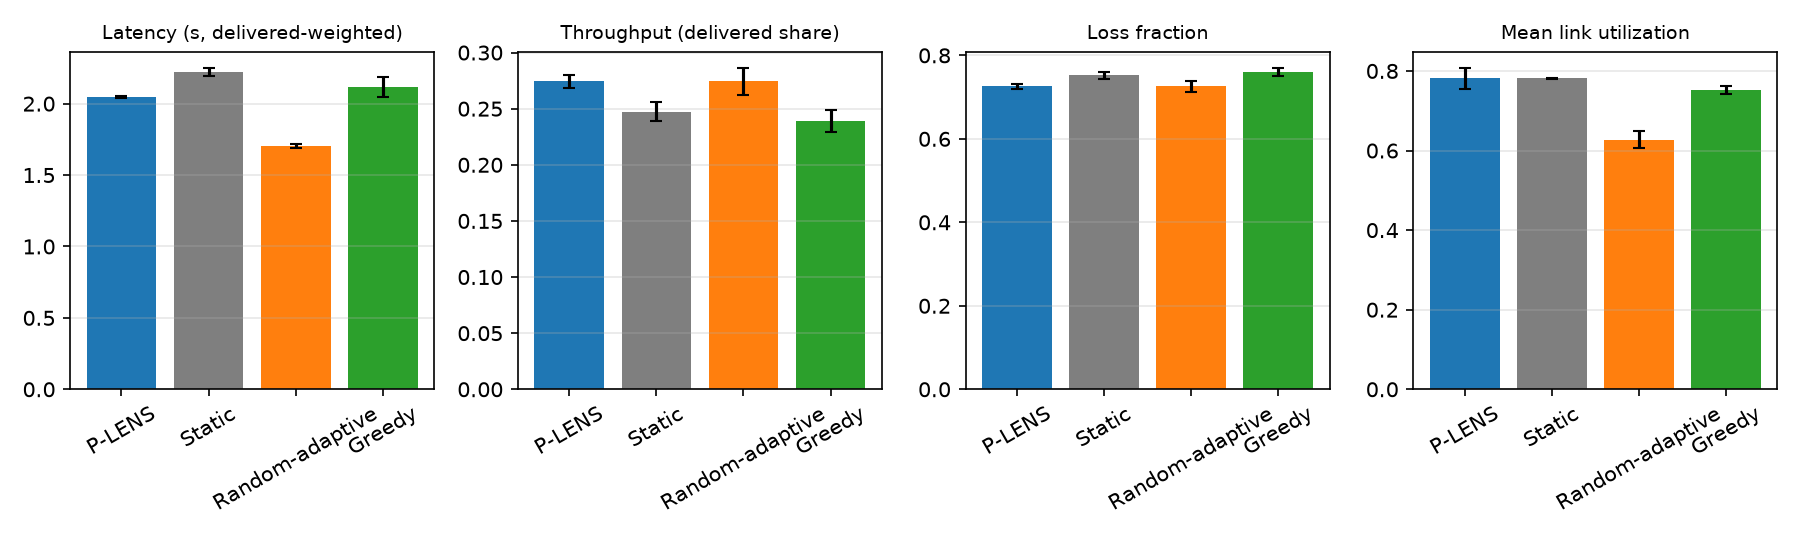
\includegraphics[width=0.95\textwidth]{policy_bars.png}
\caption{Aggregate mean $\pm$ 95\% CI per policy for latency, throughput, loss
and congestion, computed from the saved experiment summary.}
\label{fig:policybars}
\end{figure}

\begin{figure}[t]
\centering
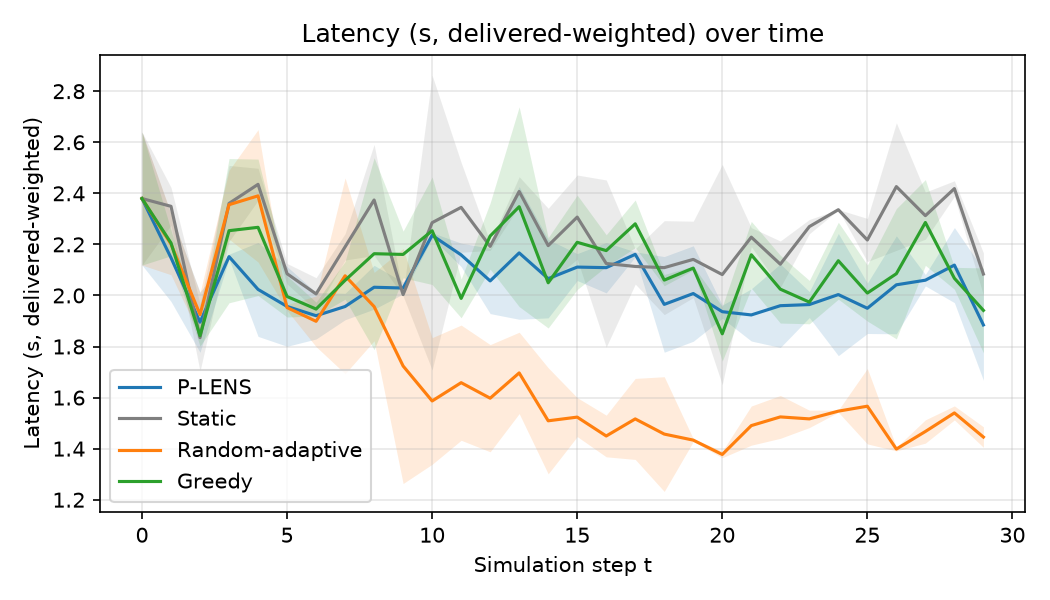
\includegraphics[width=0.95\textwidth]{timeseries_latency.png}
\caption{Latency over simulation steps (mean $\pm$ 95\% CI across seeds) for the
four policies.}
\label{fig:timeseries}
\end{figure}

\subsection{Ablations}
\label{sec:res-ablations}

Table~\ref{tab:ablations} and Figure~\ref{fig:ablationbars} show the ablation
study (3 seeds). Disabling the \emph{debt} mechanism is the most destructive:
without accumulated, unresolved pressure the controller almost never acts
($\approx$3 mutations total) and mean latency more than doubles. Disabling the
\emph{budget} drives the network to the per-step ceiling
($4\times120=480$ mutations) and yields the lowest latency, confirming that the
budget buys stability at a latency cost, and that connectivity occasionally
lapses when the budget cannot throttle it ($\text{connected}\approx0.997$).
Disabling \emph{credit} changes little in this configuration, and disabling
\emph{ML} leaves the metrics numerically unchanged, consistent with the
integration caveat discussed in \S\ref{sec:limitations}.

\begin{table}[t]
\caption{Ablations (3 seeds), mean $\pm$ 95\% CI. ``Mutations'' is the total
count over the run; ``Conn.'' the mean connected fraction.}
\label{tab:ablations}
\centering\small
\begin{tabular}{lcccc}
\toprule
Variant & Latency (ms) & Loss & Mutations & Conn. \\
\midrule
\texttt{none}      & $1.75 \pm 0.16$ & 0.939 & 81.3 & 1.000 \\
\texttt{no\_ml}    & $1.75 \pm 0.16$ & 0.939 & 81.3 & 1.000 \\
\texttt{no\_debt}  & $3.27 \pm 0.08$ & 0.949 & 3.0  & 1.000 \\
\texttt{no\_credit}& $1.82 \pm 0.17$ & 0.939 & 81.7 & 1.000 \\
\texttt{no\_budget}& $1.47 \pm 0.14$ & 0.937 & 480  & 0.997 \\
\bottomrule
\end{tabular}
\end{table}

\begin{figure}[t]
\centering
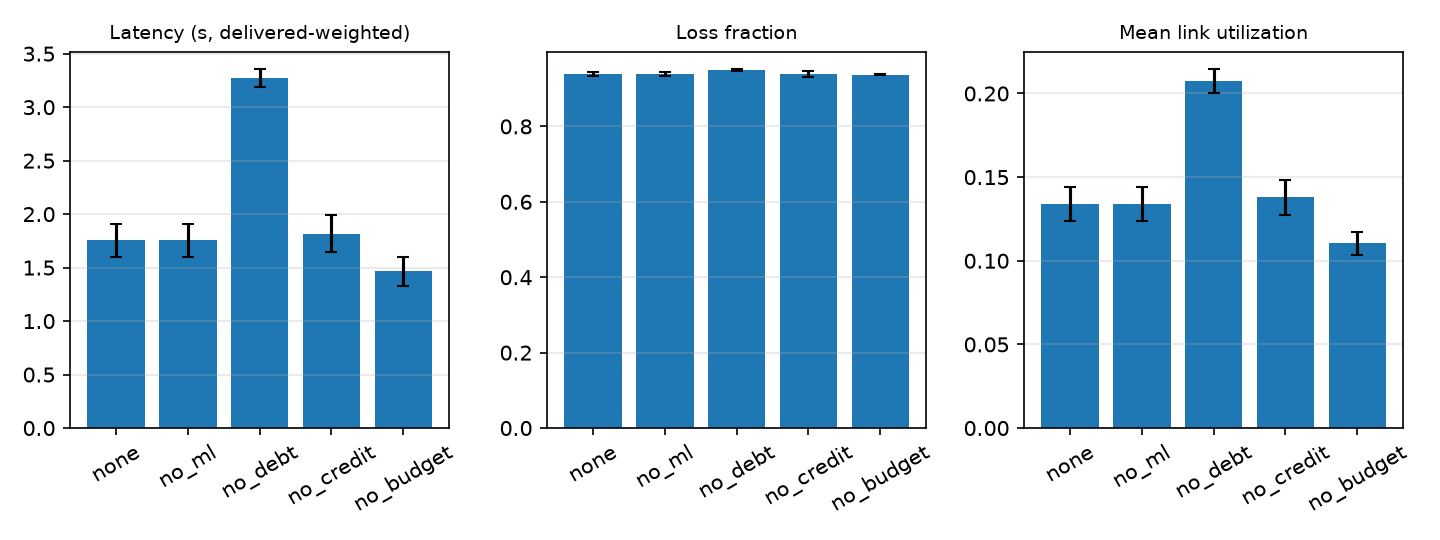
\includegraphics[width=0.95\textwidth]{ablation_bars.png}
\caption{Ablation summary: mean $\pm$ 95\% CI of latency, loss and congestion
per variant.}
\label{fig:ablationbars}
\end{figure}

\subsection{Topology evolution}
\label{sec:res-topology}

Figure~\ref{fig:topology} shows $G_t$ at four snapshots under a fixed layout, so
added edges (green) and removed edges (dashed red) read as motion rather than
layout reshuffles. P-LENS tends to add edges near congested endpoints and prune
idle ones, leaving the graph connected throughout.

\begin{figure}[t]
\centering
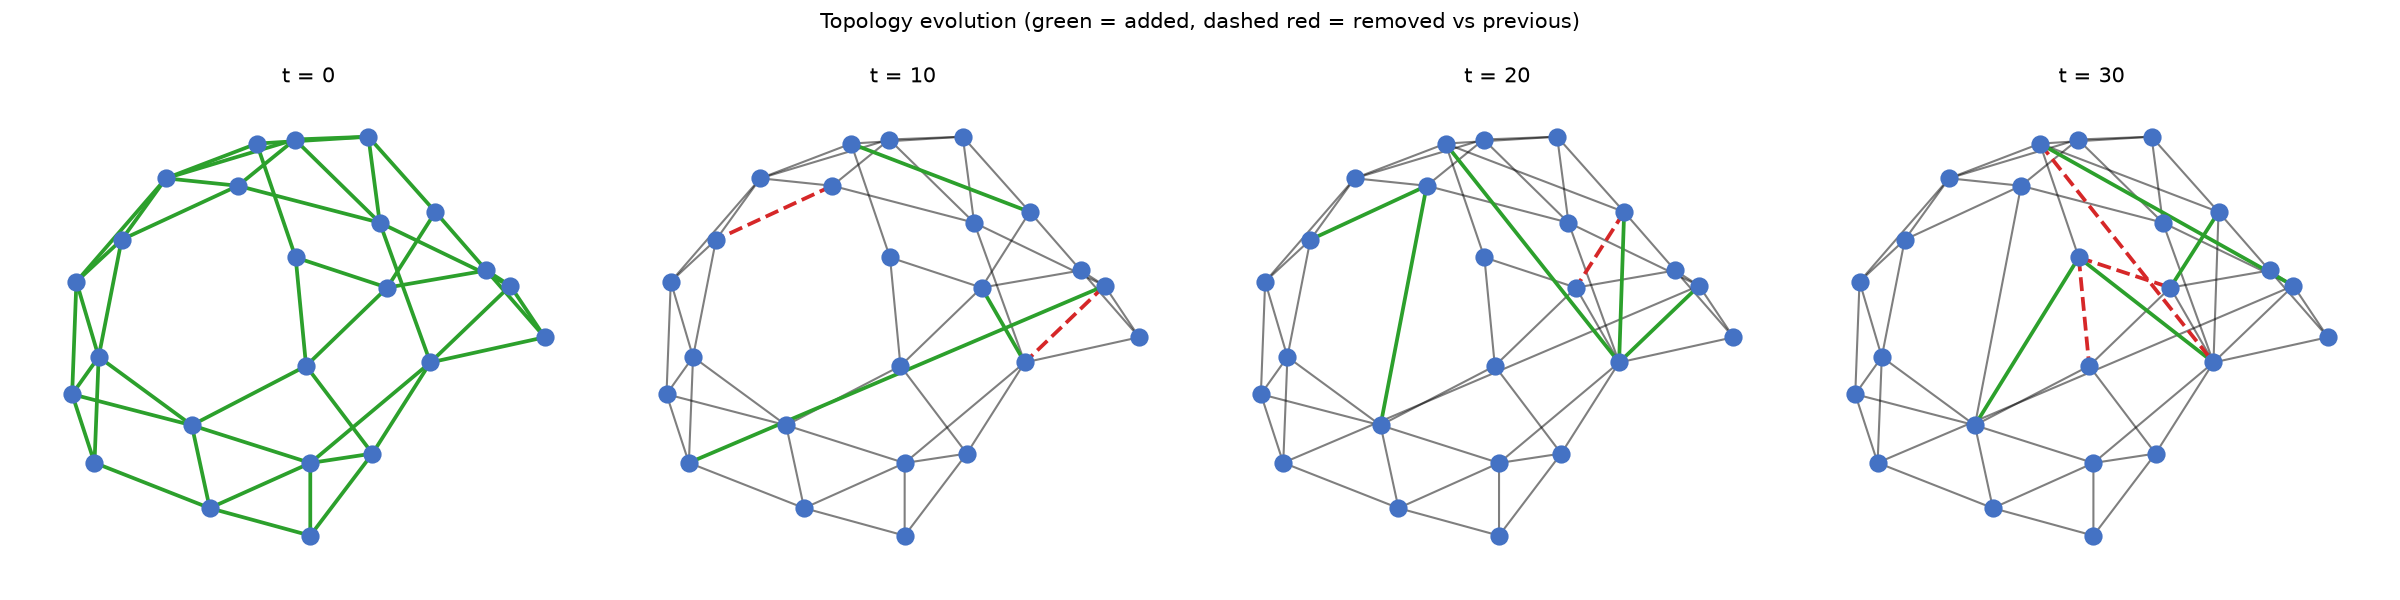
\includegraphics[width=0.95\textwidth]{topology_evolution.png}
\caption{Topology evolution: green = added, dashed red = removed relative to the
previous snapshot.}
\label{fig:topology}
\end{figure}

\subsection{Machine-learning stress classification}
\label{sec:res-ml}

Table~\ref{tab:ml} reports the GRU classifier on the CIC-IDS2017 test split
(Thursday). It reaches 0.940 accuracy and 0.902 macro-F1, beating a persistence
baseline (macro-F1 0.881) and a majority-class baseline (0.444). The validation
macro-F1 rises to $\approx$0.912 (Figure~\ref{fig:train}). We flag in
\S\ref{sec:limitations} that the current input tensor includes the per-window
attack indicator, so this figure is best read as an upper bound rather than a
leakage-free estimate.

\begin{table}[t]
\caption{GRU stress classifier on CIC-IDS2017 (Thursday test split, 913
windows).}
\label{tab:ml}
\centering\small
\begin{tabular}{lcccc}
\toprule
Class & Precision & Recall & F1 & Support \\
\midrule
Normal & 0.95 & 0.98 & 0.96 & 729 \\
Attack & 0.90 & 0.79 & 0.84 & 184 \\
\midrule
Macro avg & 0.92 & 0.88 & 0.90 & 913 \\
Accuracy  & \multicolumn{4}{c}{0.940} \\
\bottomrule
\end{tabular}
\end{table}

\begin{figure}[t]
\centering
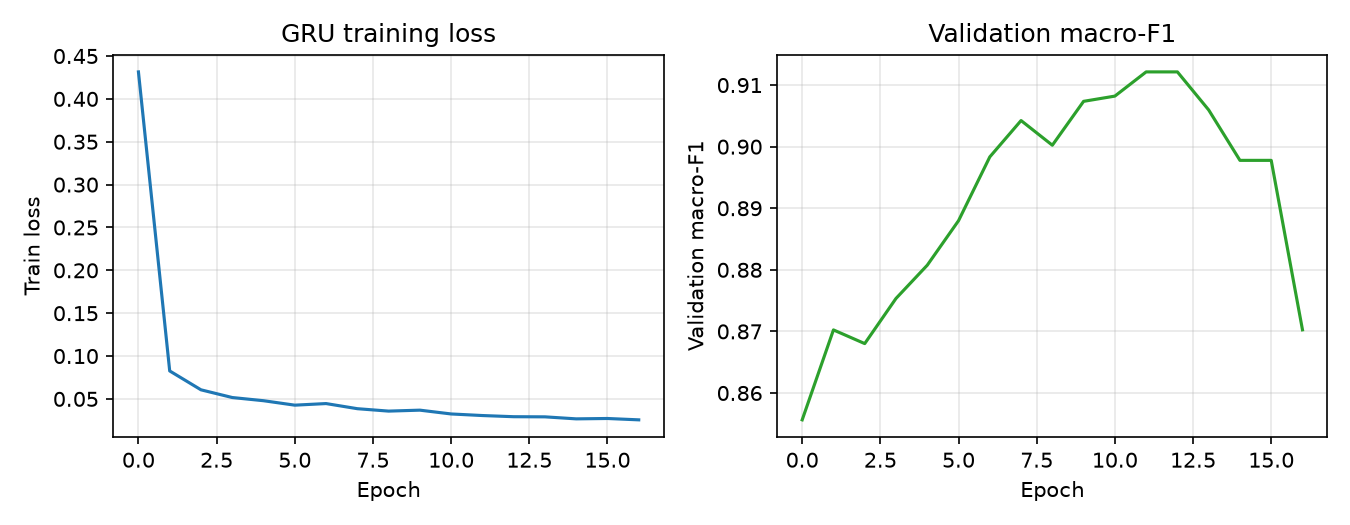
\includegraphics[width=0.9\textwidth]{training_curves.png}
\caption{GRU training loss and validation macro-F1 per epoch.}
\label{fig:train}
\end{figure}

%-=-=-=-=-=-=-=-=-=-=-=-=-=-=-=-=-=-=-=-=-=-=-=-=-=-=-=-=-=-=-=-=-=-=-=-
\section{Threats to Validity and Limitations}
\label{sec:limitations}

We state the limitations explicitly, since they qualify every number above.

\begin{itemize}
\item \textbf{Simulation-only counterfactual.} The delayed gain is computed by
reversing a mutation on the same simulated demand. A deployed network cannot
undo history; the counterfactual is an oracle, and the credit signal it produces
is optimistic by construction.
\item \textbf{Few seeds and overlapping CIs.} The reported demo runs use three
seeds; confidence bands overlap between P-LENS and the random-adaptive baseline,
so latency advantages within a single seed should not be over-interpreted. The
paired Wilcoxon test on three pairs is under-powered.
\item \textbf{ML input leakage.} In the current implementation the classifier's
input vector contains the per-window attack indicator (feature index 9), which
is also the source of the label. This inflates the reported accuracy; a
leakage-free variant (nine traffic features only) is expected to score lower and
is left as future work.
\item \textbf{ML integration is currently inert.} The stress-to-scale map still
uses legacy \texttt{Low/Medium/High} keys, so the two-class predicted label
always falls through to the neutral scale ($\text{scale}=1$). Consequently the
\texttt{no\_ml} ablation is identical to the full model, and the forecaster does
not yet influence the simulation.
\item \textbf{Metrics are proxies.} Throughput, latency and loss come from a
single-pass shortest-path model with a normalised M/M/1 queue term and a
per-flow bottleneck share; these are bottleneck proxies, not packet-level
measurements.
\item \textbf{Fixed node set and mutation vocabulary.} Only edges change; nodes
are never added or removed, and rewiring moves a single endpoint.
\item \textbf{Data-derived endpoints.} When real datasets are used, flow
endpoints are hashed from ports/services rather than observed, so the demand
matrix is a plausible replay, not ground truth about the traced topology.
\end{itemize}

%-=-=-=-=-=-=-=-=-=-=-=-=-=-=-=-=-=-=-=-=-=-=-=-=-=-=-=-=-=-=-=-=-=-=-=-
\section{Conclusion}
\label{sec:conclusion}

We presented P-LENS, a framework for evolving communication-network topology
driven by plasticity pressure, accumulated debt and a global mutation budget,
with delayed counterfactual evaluation and per-edge credit. P-LENS adapts more
conservatively than a random-adaptive baseline while beating static and greedy
policies on latency, and its mechanisms are individually ablatable. The current
prototype also exposes several clear integration gaps---most importantly a
machine-learning input leak and an inert stress-to-scale map---which we have
documented rather than hidden. Natural next steps are a leakage-free classifier,
a working stress-to-scale coupling, a packet-level or queueing-network
simulator, and a larger multi-seed study with the paired test fully powered.

%-=-=-=-=-=-=-=-=-=-=-=-=-=-=-=-=-=-=-=-=-=-=-=-=-=-=-=-=-=-=-=-=-=-=-=-

\subsubsection*{Acknowledgements.}
This work was carried out as a class project by Team~5 at VIT-AP University,
under the supervision of G.~Deepthi (Faculty, VIT-AP University). The authors
thank the course staff and the anonymous reviewers for their feedback. No
external funding was used.

\bibliographystyle{splncs04}
\bibliography{references}

\end{document}
